% Gallery figure source
% Summary: Four common ancestry and contact objects in infectious disease work. Contact networks describe possible contacts, transmission trees describe who infected whom, pathogen phylogenies describe genome ancestry under a tree assumption, and phylogenetic networks allow reticulate events such as recombination, reassortment, hybridisation, or horizontal gene transfer.
\documentclass[tikz,border=6pt]{standalone}
% Shared color palette
\usepackage[T1]{fontenc}
\usepackage[utf8]{inputenc}
\usepackage{lmodern}
\usepackage{microtype}
\usepackage{amsmath,amssymb,mathtools}
\usepackage{xcolor}
\usepackage{tikz}
\usetikzlibrary{arrows.meta,positioning,calc,fit,backgrounds,decorations.pathreplacing,shapes.geometric,shadows.blur}

\definecolor{mainblue}{RGB}{42,85,132}
\definecolor{deepgreen}{RGB}{30,105,70}
\definecolor{burntorange}{RGB}{190,90,25}
\definecolor{softgray}{RGB}{245,246,248}
\definecolor{darkgray}{RGB}{70,70,70}
\definecolor{violet}{RGB}{110,70,150}

\newcommand{\given}{\,|\,}
\newcommand{\Ne}{N_{e}}
\newcommand{\ARG}{\mathrm{ARG}}
\newcommand{\MRCA}{\mathrm{MRCA}}
\newcommand{\GMRCA}{\mathrm{GMRCA}}

% Shared TikZ styles
\tikzset{
  tip/.style={circle,fill=black,inner sep=1.6pt},
  nodept/.style={circle,fill=black,inner sep=1.4pt},
  sampled/.style={rectangle,fill=black,inner sep=2.2pt},
  branch/.style={line width=0.8pt},
  retic/.style={circle,draw=burntorange,fill=burntorange!25,line width=0.8pt,inner sep=2.0pt},
  event/.style={circle,draw=mainblue,fill=mainblue!15,line width=0.8pt,inner sep=1.8pt},
  arr/.style={-{Latex[length=2.0mm]},line width=0.8pt},
  faint/.style={line width=0.7pt,draw=gray!55},
  parentedge/.style={-{Latex[length=2.0mm]},line width=0.9pt,draw=burntorange},
  treeedge/.style={-{Latex[length=2.0mm]},line width=0.9pt,draw=black},
  segment/.style={line width=4pt,line cap=round},
  dashedretic/.style={-{Latex[length=2.0mm]},line width=0.9pt,draw=burntorange,dashed}
}


\begin{document}
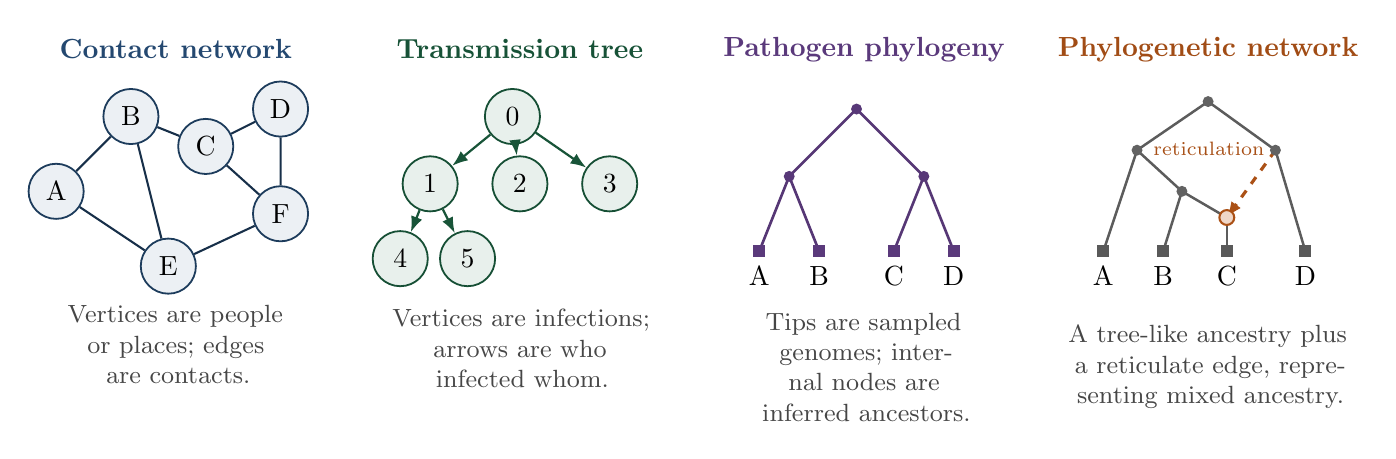
\begin{tikzpicture}[
  scale=0.95,
  arr/.style={-{Latex[length=2mm]},line width=.8pt,draw=deepgreen!80!black},
  contactedge/.style={line width=.75pt,draw=mainblue!55!black},
  branch/.style={line width=.9pt,draw=darkgray!88},
  phybranch/.style={line width=.95pt,draw=violet!78!black},
  retic/.style={-{Latex[length=2mm]},line width=1.15pt,dashed,draw=burntorange!90!black},
  nodept/.style={circle,fill=darkgray!85,inner sep=1.4pt},
  phynode/.style={circle,fill=violet!80!black,inner sep=1.4pt},
  sampled/.style={rectangle,fill=darkgray!90,inner sep=2.2pt},
  contactnode/.style={circle,draw=mainblue!70!black,fill=mainblue!9,minimum size=7mm,line width=.65pt},
  transnode/.style={circle,draw=deepgreen!75!black,fill=deepgreen!10,minimum size=7mm,line width=.65pt},
  paneltitle/.style={font=\bfseries},
  paneltext/.style={text width=3.4cm,align=center,font=\small,text=darkgray}
]

  \node[paneltitle,text=mainblue!85!black] at (1.6,2.9) {Contact network};

  \foreach \x/\y/\n in {0/1/A,1/2/B,2/1.6/C,3/2.1/D,1.5/0/E,3/0.7/F}{
    \node[contactnode] (c\n) at (\x,\y) {\n};
  }

  \draw[contactedge] (cA)--(cB)--(cC)--(cD)--(cF)--(cE)--(cA);
  \draw[contactedge] (cB)--(cE);
  \draw[contactedge] (cC)--(cF);

  \node[paneltext,text width=3.2cm] at (1.6,-1.05)
    {Vertices are people or places; edges are contacts.};

  \begin{scope}[xshift=4.6cm]

    \node[paneltitle,text=deepgreen!78!black] at (1.6,2.9) {Transmission tree};

    \node[transnode] (t0) at (1.5,2) {0};
    \node[transnode] (t1) at (0.4,1.1) {1};
    \node[transnode] (t2) at (1.6,1.1) {2};
    \node[transnode] (t3) at (2.8,1.1) {3};
    \node[transnode] (t4) at (0.0,0.1) {4};
    \node[transnode] (t5) at (0.9,0.1) {5};

    \draw[arr] (t0)--(t1);
    \draw[arr] (t0)--(t2);
    \draw[arr] (t0)--(t3);
    \draw[arr] (t1)--(t4);
    \draw[arr] (t1)--(t5);

    \node[paneltext] at (1.6,-1.10)
      {Vertices are infections; arrows are who infected whom.};
  \end{scope}

  \begin{scope}[xshift=9.2cm]
    \node[paneltitle,text=violet!82!black] at (1.6,2.9) {Pathogen phylogeny};

    \coordinate (r) at (1.5,2.1);
    \coordinate (a) at (0.6,1.2);
    \coordinate (b) at (2.4,1.2);
    \coordinate (c) at (0.2,0.2);
    \coordinate (d) at (1.0,0.2);
    \coordinate (e) at (2.0,0.2);
    \coordinate (f) at (2.8,0.2);

    \draw[phybranch] (r)--(a)--(c);
    \draw[phybranch] (a)--(d);
    \draw[phybranch] (r)--(b)--(e);
    \draw[phybranch] (b)--(f);

    \foreach \p/\lab in {c/A,d/B,e/C,f/D}{
      \node[rectangle,fill=violet!82!black,inner sep=2.2pt] at (\p) {};
      \node[below=2pt] at (\p) {\lab};
    }

    \foreach \p in {r,a,b}{
      \node[phynode] at (\p) {};
    }

    \node[paneltext] at (1.6,-1.35)
      {Tips are sampled genomes; internal nodes are inferred ancestors.};
  \end{scope}

  \begin{scope}[xshift=13.8cm]

    \node[paneltitle,text=burntorange!85!black] at (1.6,2.9) {Phylogenetic network};

    \coordinate (nr) at (1.6,2.2);
    \coordinate (nl) at (0.65,1.55);
    \coordinate (nv) at (2.50,1.55);
    \coordinate (nu) at (1.25,1.00);
    \coordinate (nh) at (1.85,0.65);
    \coordinate (nA) at (0.20,0.20);
    \coordinate (nB) at (1.00,0.20);
    \coordinate (nC) at (1.85,0.20);
    \coordinate (nD) at (2.90,0.20);

    \draw[branch] (nr)--(nl);
    \draw[branch] (nr)--(nv);
    \draw[branch] (nl)--(nA);
    \draw[branch] (nl)--(nu);
    \draw[branch] (nu)--(nB);
    \draw[branch] (nu)--(nh);
    \draw[branch] (nh)--(nC);
    \draw[branch] (nv)--(nD);

    \draw[retic] (nv)--(nh);

    \foreach \p in {nr,nl,nv,nu}{
      \node[nodept] at (\p) {};
    }

    \node[circle,draw=burntorange!90!black,fill=burntorange!24,line width=.75pt,inner sep=1.9pt] at (nh) {};

    \foreach \p/\lab in {nA/A,nB/B,nC/C,nD/D}{
      \node[rectangle,fill=darkgray!90,inner sep=2.2pt] at (\p) {};
      \node[below=2pt] at (\p) {\lab};
    }

    \node[font=\scriptsize,text=burntorange!88!black,align=center] at (1.61,1.57)
      {reticulation};

    \node[paneltext,text width=3.6cm] at (1.6,-1.35)
      {A tree-like ancestry plus a reticulate edge, representing mixed ancestry.};
  \end{scope}
\end{tikzpicture}
\end{document}
